\documentclass[dvipsnames,crop=true]{standalone}
\usepackage{tikz}
\usepackage{etoolbox}
\usepackage{pgfplots}
\usetikzlibrary{calc,external,intersections,fillbetween}
\begin{document}

  \tikzsetnextfilename{geo_binning}
  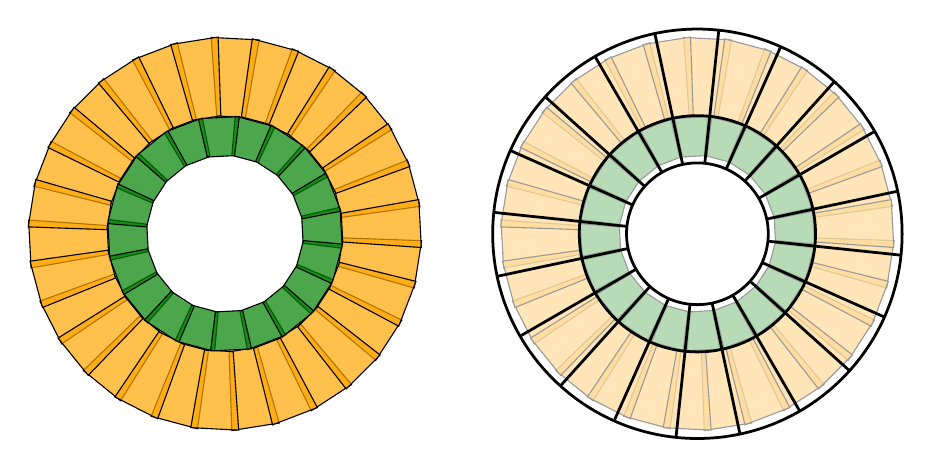
\begin{tikzpicture}[scale=1.0]

    \pgfdeclarelayer{top}
    \pgfdeclarelayer{bottom}
    \pgfdeclarelayer{bins}
    \pgfsetlayers{top,bottom,bins,main}

    \foreach \x/\l in {-3/a, 3/b}{
      \begin{scope}[shift={(\x, 0)}]
        \foreach \nlines/\rmin/\rmax/\w/\color/\offset in%
        {20/1/1.5/20/Green/-5, 30/1.5/2.5/14/Orange/10}{
          \pgfmathsetmacro{\amax}{\nlines - 1}
          \foreach \a in {0,...,\amax}{
            \begin{pgfonlayer}{\ifnumodd{\a}{top}{bottom}}
              \draw [fill=\color,fill opacity=0.7] let \n{left}={\a * 360 / \nlines + \offset}, \n{right}={\n{left}-\w} in%
              (\n{left}:\rmin) -- (\n{left}:\rmax) -- (\n{right}:\rmax) -- (\n{right}:\rmin) -- (\n{left}:\rmin);
            \end{pgfonlayer}
          }
        }
        % \node[] () at (0, -3) {\small (\l)};
      \end{scope}
    }

    \begin{scope}[shift={(3, 0)}]
      \pgfmathsetmacro{\ndiv}{20}
      \pgfmathsetmacro{\ndivmn}{\ndiv-1}
      \pgfmathsetmacro{\offset}{-6}
      \def\rmin{0.9}
      \def\rmax{2.6}
      \begin{pgfonlayer}{bins}

      \path [name path=inner] (0,0) circle (\rmin);
      \path [name path=outer] (0,0) circle (\rmax);
      \tikzfillbetween[of=inner and outer]{white, opacity=0.6};

      \foreach \a in {0,...,\ndivmn}{
          \draw [line width=1pt] let \n{left}={\a * 360 / \ndiv + \offset} in (\n{left}:\rmin) -- (\n{left}:\rmax);
      }

      \draw [line width=1pt] (0,0) circle (\rmin);
      \draw [line width=1pt] (0,0) circle (1.5);
      \draw [line width=1pt] (0,0) circle (\rmax);
      \end{pgfonlayer}
    \end{scope}

  \end{tikzpicture}

\end{document}